\documentclass[aspectratio=169,10pt]{beamer}

\usetheme{Madrid}
\usecolortheme{default}
\setbeamertemplate{navigation symbols}{}
\setbeamertemplate{footline}[frame number]

\usepackage{booktabs}
\usepackage{graphicx}
\usepackage{tikz}
\usepackage[T1]{fontenc}
\usepackage{lmodern}
\usepackage{textcomp}
\usepackage{adjustbox}

\title{Migration Mortality on the Central Mediterranean Route}
\subtitle{Evidence from Weather Variation}
\author{Giorgio Coppola}
\institute{Hertie School --- Master of Data Science}
\date{April 2026}

\begin{document}

\begin{frame}
\titlepage
\end{frame}

% ═════════════════════════════════════════════════════════
\begin{frame}{Motivation and Identification Challenge}

\textbf{Question.} How did the dangerousness for migrants crossing the Central
Mediterranean evolve across policy periods?

\vspace{0.5em}
\textbf{Why it is hard.} Total deaths depend on many moving pieces at once:
\begin{itemize}
  \item \emph{Volume}: departures volume change constantly depending on many push and pull factors (plus no departure variable)
  \item \emph{Composition}: inflatable share and boat crowding change
  over time
  \item \emph{"Smuggling Behaviour"}: smugglers decide when to launch boats depending on many unpredictable factos
  \item \emph{Weather}: daily sea conditions are exogenous but volatile
  \item \emph{Institutions}: SAR coverage (Mare Nostrum $\to$ NGO SAR $\to$ LCG $\to$ NGO block) shifts repeatedly across 2013--present
\end{itemize}

\vspace{0.5em}
A before/after count comparison confounds all of these. We need an identifier
that is \emph{fixed by construction} and does not move with the policy.

\end{frame}

% ═════════════════════════════════════════════════════════
\begin{frame}{Identification Strategy}

\textbf{Significant wave height (SWH)} is a constant physical hazard. How this hazard translates into deaths across periods?

\textbf{Main period specification:} Pre-2017, Post-2017; multi-period analysis 

\vspace{0.5em}
\begin{columns}[T]
\begin{column}{0.48\textwidth}
\textbf{Estimand:} the change in the SWH--mortality gradient.
\[
\Delta\beta = \beta^{\text{post}}_{\text{SWH}} - \beta^{\text{pre}}_{\text{SWH}}
\]
Identified off within-month variation in weather (using month-year FE, absorbing t.v. confounders)
\end{column}
\begin{column}{0.48\textwidth}
\textbf{Hypothesis:}
\begin{itemize}
  \item Weather: unchanged
  \item SAR: removed, provided "guardrails"
\end{itemize}
$\Rightarrow$ the route became more dangerous \emph{per unit of exposure}.
\end{column}
\end{columns}

\vspace{0.5em}
\textbf{Primary specification:}
\[
n^{\text{deaths}}_{t} \;=\; \beta_{1}\,\text{SWH}^{\text{prev5d}}_{t}
\;+\; \beta_{3}\,\text{SWH}^{\text{prev5d}}_{t}\!\times\!\text{Post}_t
\;+\; \gamma_{m(t)} \;+\; \varepsilon_{t}
\]

\vspace{0.4em}
\footnotesize
Regresses daily deaths on 5-day mean SWH and its interaction with a
post-policy indicator, conditional on month-year fixed effects --- so
$\beta_3$ measures how the within-month weather-to-deaths slope changes after
the policy, with all monthly-frequency confounders (volume, composition,
institutions, season) absorbed by the FE.

\end{frame}

% ═════════════════════════════════════════════════════════
\begin{frame}{Data and Sample}

\textbf{Daily panel, 2014-01-15 to 2023-05-31 ($N = 3{,}424$ days).}

\vspace{0.3em}
\begin{table}
\centering
\small
\begin{tabular}{lll}
\toprule
\textbf{Source} & \textbf{Variable} & \textbf{Notes} \\
\midrule
IOM MMP & Deaths \& missing ($n^{\text{deaths}}$) & Central Med., incident + split, drown+mixed \\
UNITED & Deaths \& missing ($n^{\text{deaths}}$) & Central Med., drown+mixed \\
ERA5 reanalysis & Prev 5-day SWH (metres) & Corridor-wide mean, $0.5^\circ$ grid \\
Frontex Themis & Daily crossing attempts & Frx persons + LCG/TCG pushbacks \\
IMO GISIS & SAR zone polygons & Libya, Tunisia, Italy, Malta \\
\bottomrule
\end{tabular}
\end{table}

\vspace{0.3em}
\textbf{Corridor delineation.} Core-corridor polygon built from ERA5 ocean cells
bounded by North-Africa/EU coastlines.

\vspace{0.3em}
\textbf{SWH.} spatial average over the corridor (each cell is highly correlated to the avg)
\end{frame}

% ═════════════════════════════════════════════════════════
\begin{frame}{ Corridor and SAR Zones}
\begin{columns}[T]
\begin{column}{0.48\textwidth}
\begin{center}
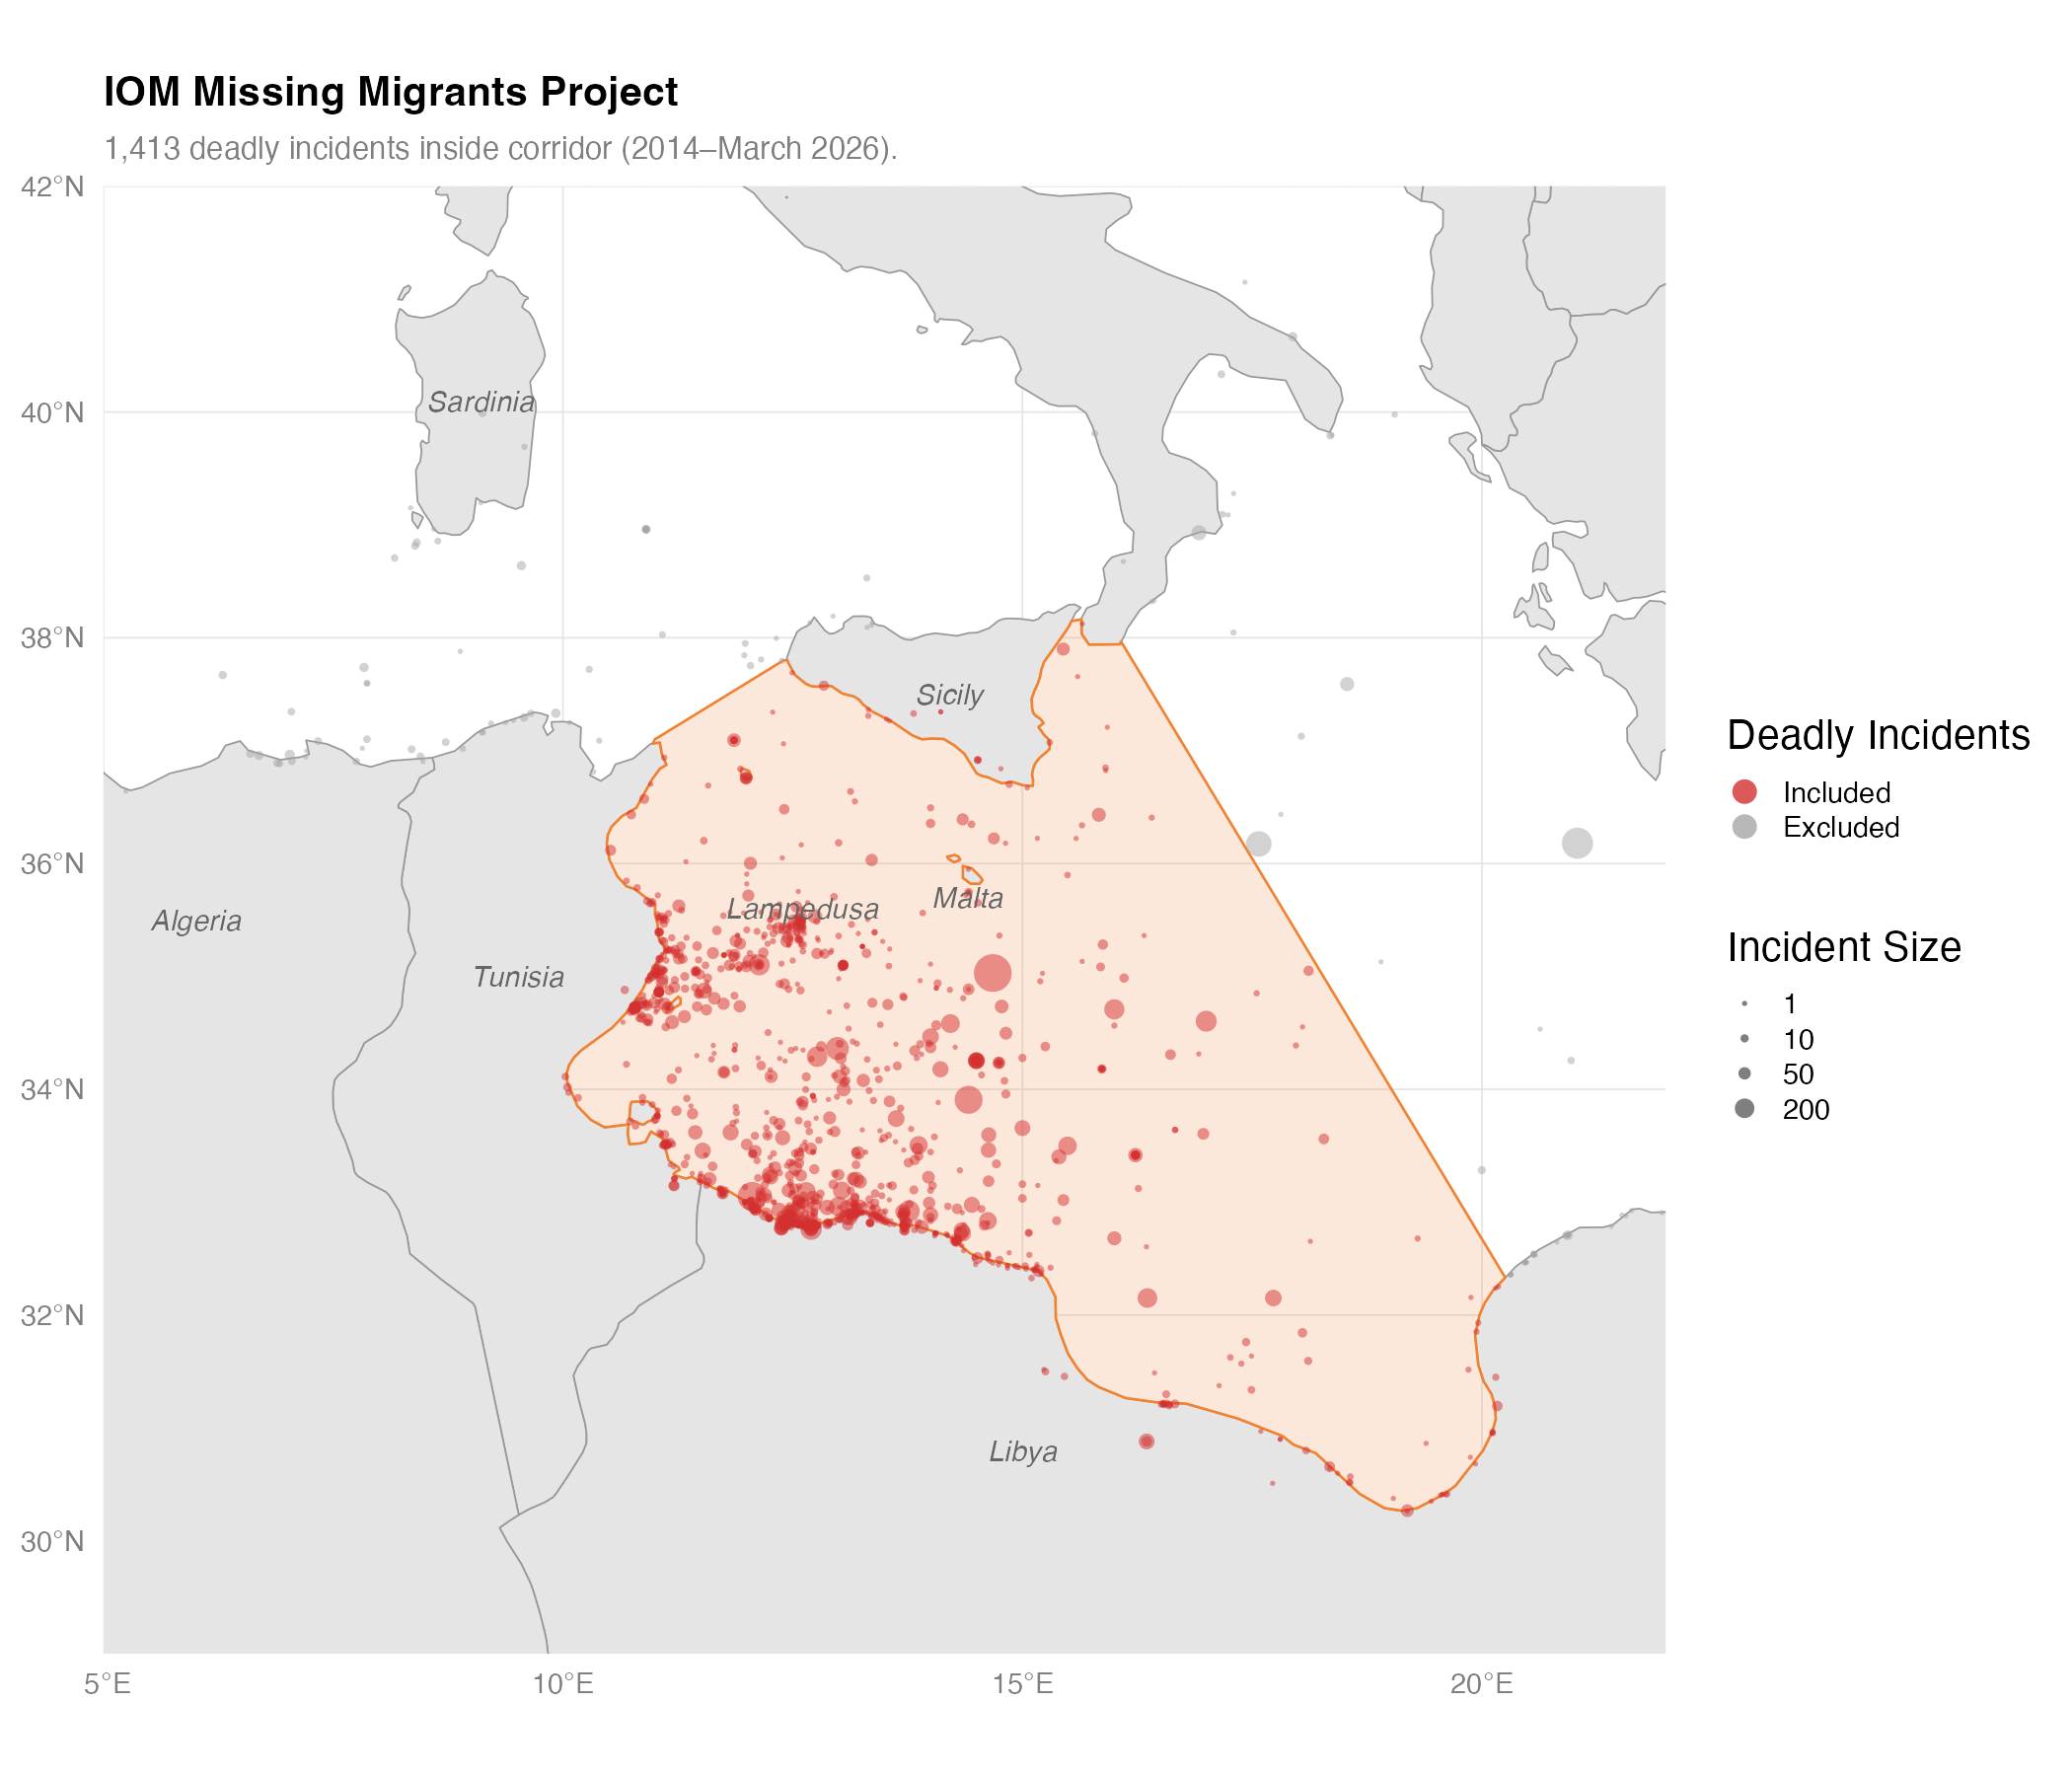
\includegraphics[width=\linewidth,height=0.8\textheight,keepaspectratio]{../../output/figures/desc_iom_incidents_map.png}
\end{center}

\end{column}
\begin{column}{0.48\textwidth}
\begin{center}
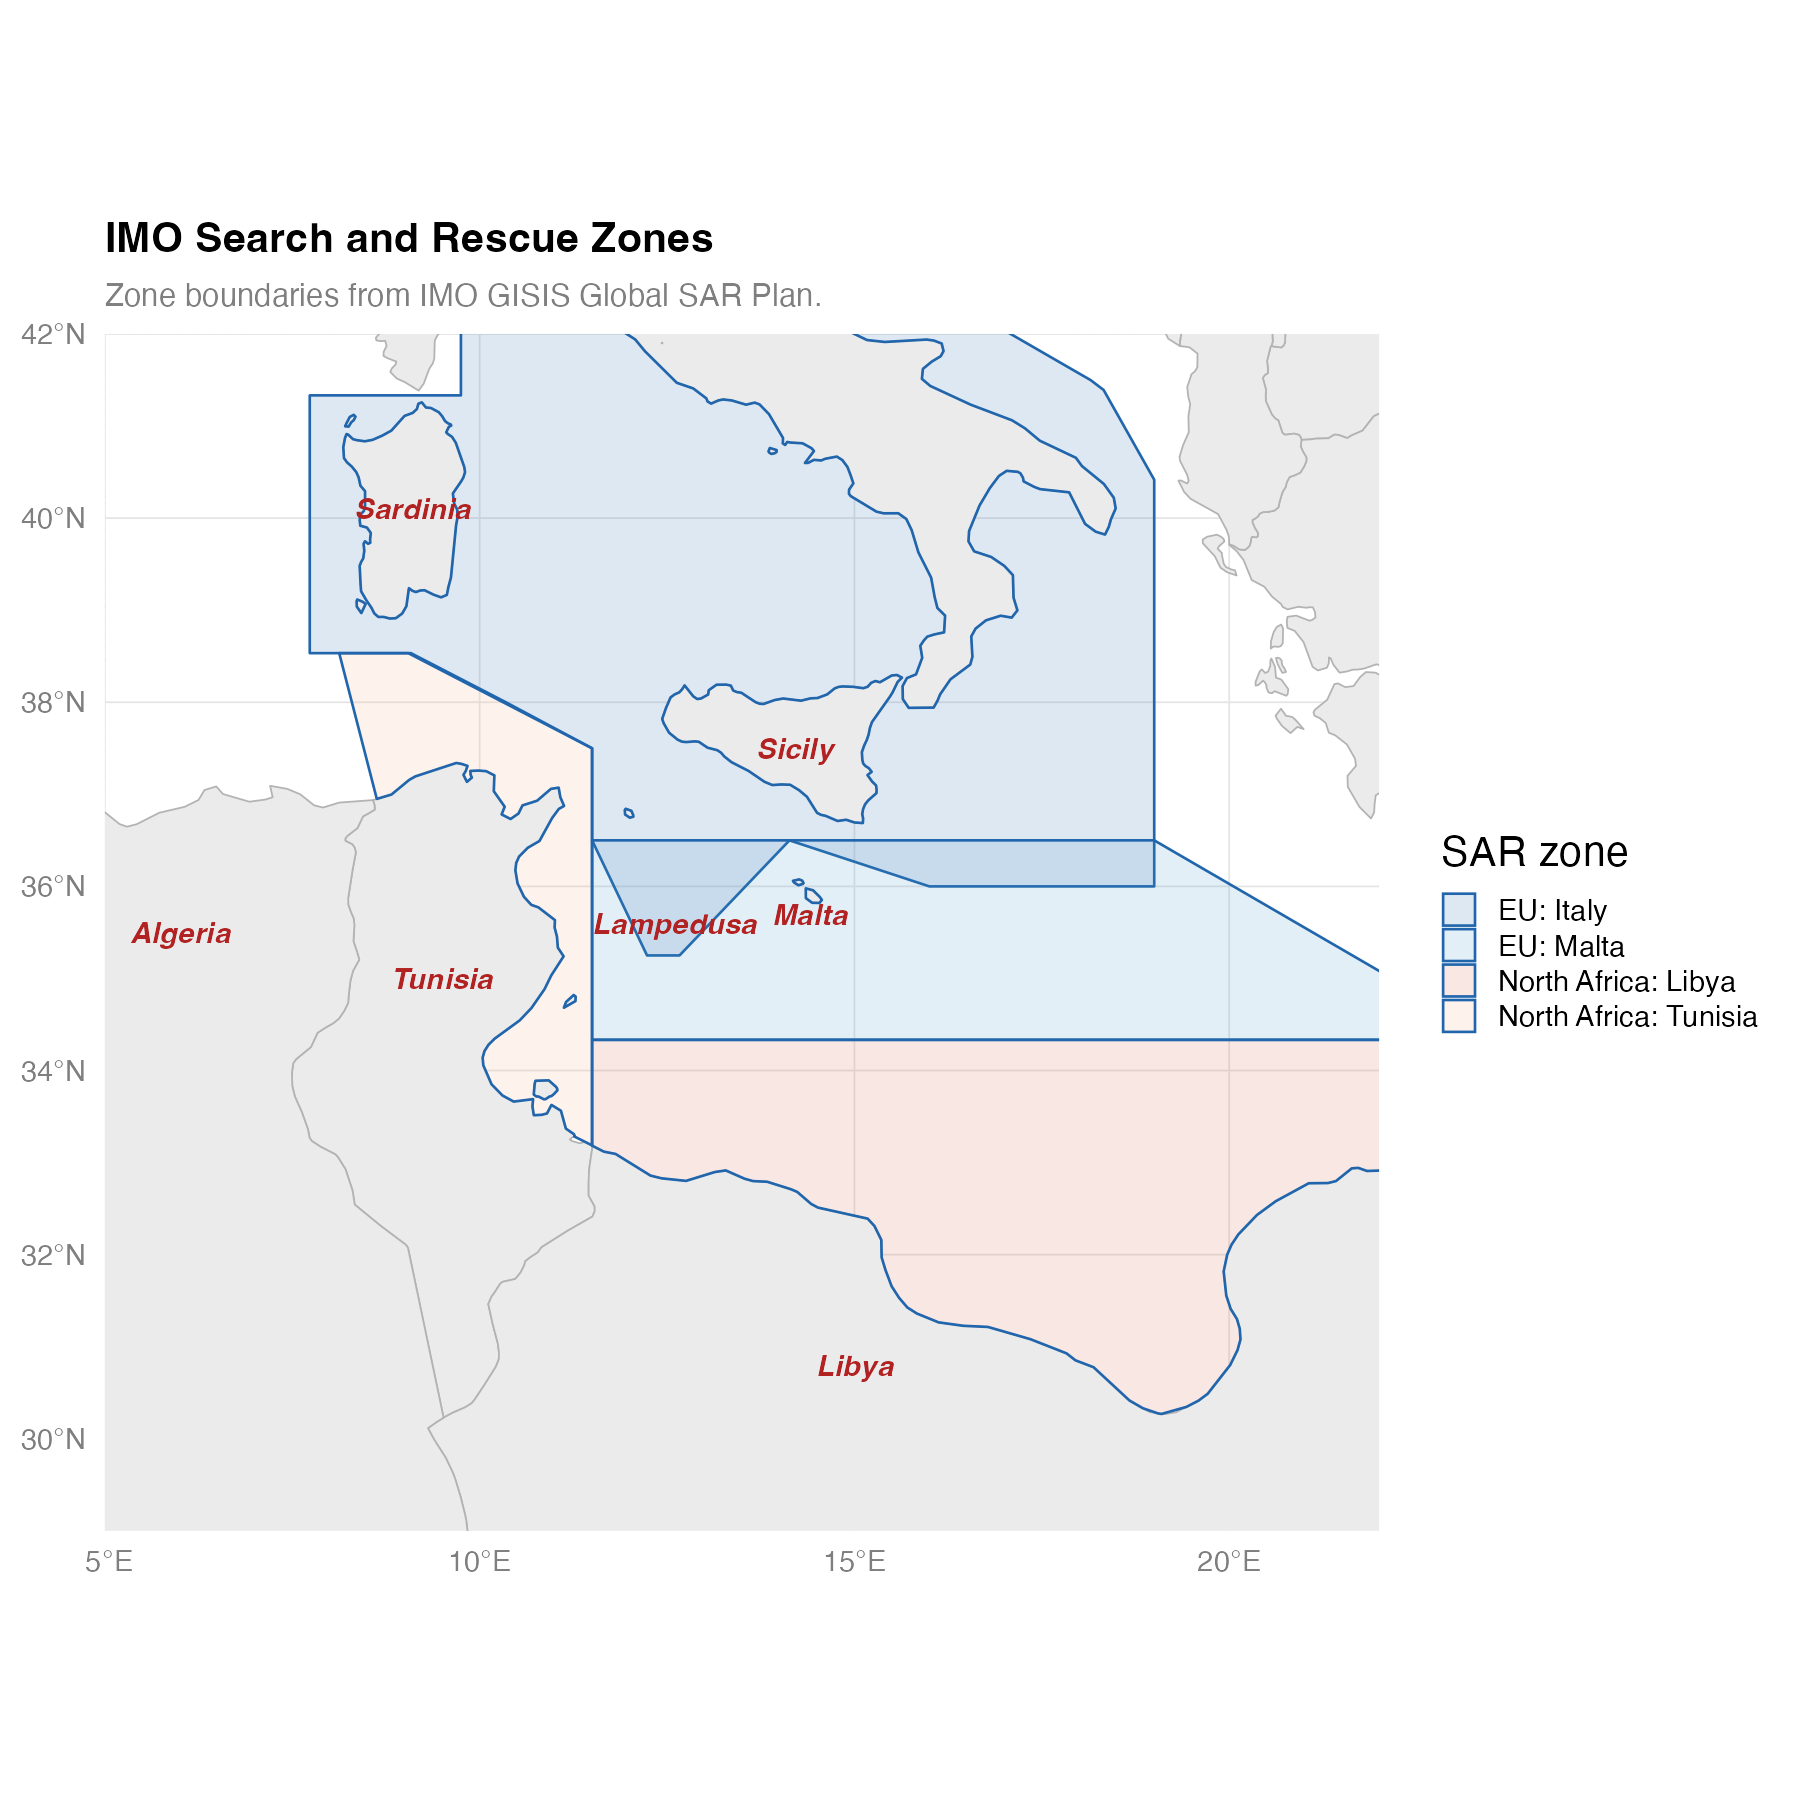
\includegraphics[width=\linewidth,height=0.8\textheight,keepaspectratio]{../../output/figures/desc_sar_zones.png}
\end{center}

\end{column}
\end{columns}
\end{frame}

% ═════════════════════════════════════════════════════════
\begin{frame}{Primary Specification --- Modelling Choices}

\[
n^{\text{deaths}}_{t} \;\sim\; \text{SWH}^{\text{prev}}_{t}
\;+\; \text{SWH}^{\text{prev}}_{t}\!\times\!\text{Post}_t
\;\mid\; \text{month-year FE}
\]

\vspace{0.3em}
\begin{columns}[T]
\begin{column}{0.48\textwidth}
\textbf{Two families:}
\begin{itemize}
  \item \textbf{Negative Binomial} (fenegbin) --- high dispersion
  \item \textbf{Poisson QMLE} (fepois) --- weaker
    assumptions 
\end{itemize}
Agreement across the two.
\end{column}
\begin{column}{0.48\textwidth}
\textbf{Standard errors:} Newey--West with lag $L=14$ (primary); also
cluster-robust on month-year.

\vspace{0.4em}
\textbf{Rate robustness:} Poisson with offset $\log(\text{attempts})$ on
days with non-zero attempts ($N=2{,}069$).

\vspace{0.4em}
\textbf{Crossing controls:} log1p of lagged 7-day and 14-day rolling means
of living crossings, included as robustness.
\end{column}
\end{columns}

\vspace{0.5em}
\footnotesize
Month-year FE absorb 51\% of 5-day SWH variance, leaving within-month weather
shocks as the identifying variation. \texttt{Post} is fully absorbed by the FE
$\Rightarrow$ identified only through the interaction.
\end{frame}

% ═════════════════════════════════════════════════════════
\begin{frame}{Primary Results}

\begin{table}
\centering
\small
\begin{tabular}{lccc}
\toprule
 & \textbf{NegBin count} & \textbf{Poisson count} & \textbf{Poisson rate (offset)} \\
\midrule
$\beta_1$ (SWH, pre-MoU)     & $-1.98^{***}$  & $-1.85^{**}$   & $-2.36^{**}$ \\
                              & $(0.60)$       & $(0.66)$       & $(0.85)$ \\
$\beta_3$ (SWH $\times$ Post) & $+2.22^{**}$   & $+2.04^{**}$   & $+2.73^{**}$ \\
                              & $(0.69)$       & $(0.72)$       & $(0.93)$ \\
\midrule
Observations                  & $3{,}286$      & $3{,}286$      & $2{,}069$ \\
Month-year FE                 & Yes            & Yes            & Yes \\
Newey--West $L=14$ SEs        & Yes            & Yes            & Yes \\
\bottomrule
\end{tabular}
\end{table}

\vspace{0.5em}
\begin{itemize}
  \item \textbf{Sign flip}: pre-MoU $\beta(\text{SWH}) = -1.98$ (rough seas $\to$ fewer deaths, consistent with SAR protection + voluntary departure cuts). Post-MoU: $-1.98 + 2.22 = +0.24$.
  \item \textbf{Agreement across families} (NegBin / Poisson / rate)
  \item \textbf{Rate model} ($n/\text{attempts}$): the per-attempt gradient moves conditional on crossing.
\end{itemize}
\end{frame}

% ═════════════════════════════════════════════════════════
\begin{frame}{Year-by-Year Gradient}

\begin{center}
\includegraphics[width=0.95\linewidth,height=0.80\textheight,keepaspectratio]{../../output/figures/20_yearly_gradient.png}
\end{center}

\footnotesize
$\beta(\text{SWH})$ by year. NegBin + Poisson, no crossing control and with
lag-7d control. Red dotted = MoU. Gradient is negative in 2014--17, roughly
zero or positive after.
\end{frame}

% ═════════════════════════════════════════════════════════
\begin{frame}{Rolling-Window $\beta$ --- Gradual Transition}

\begin{center}
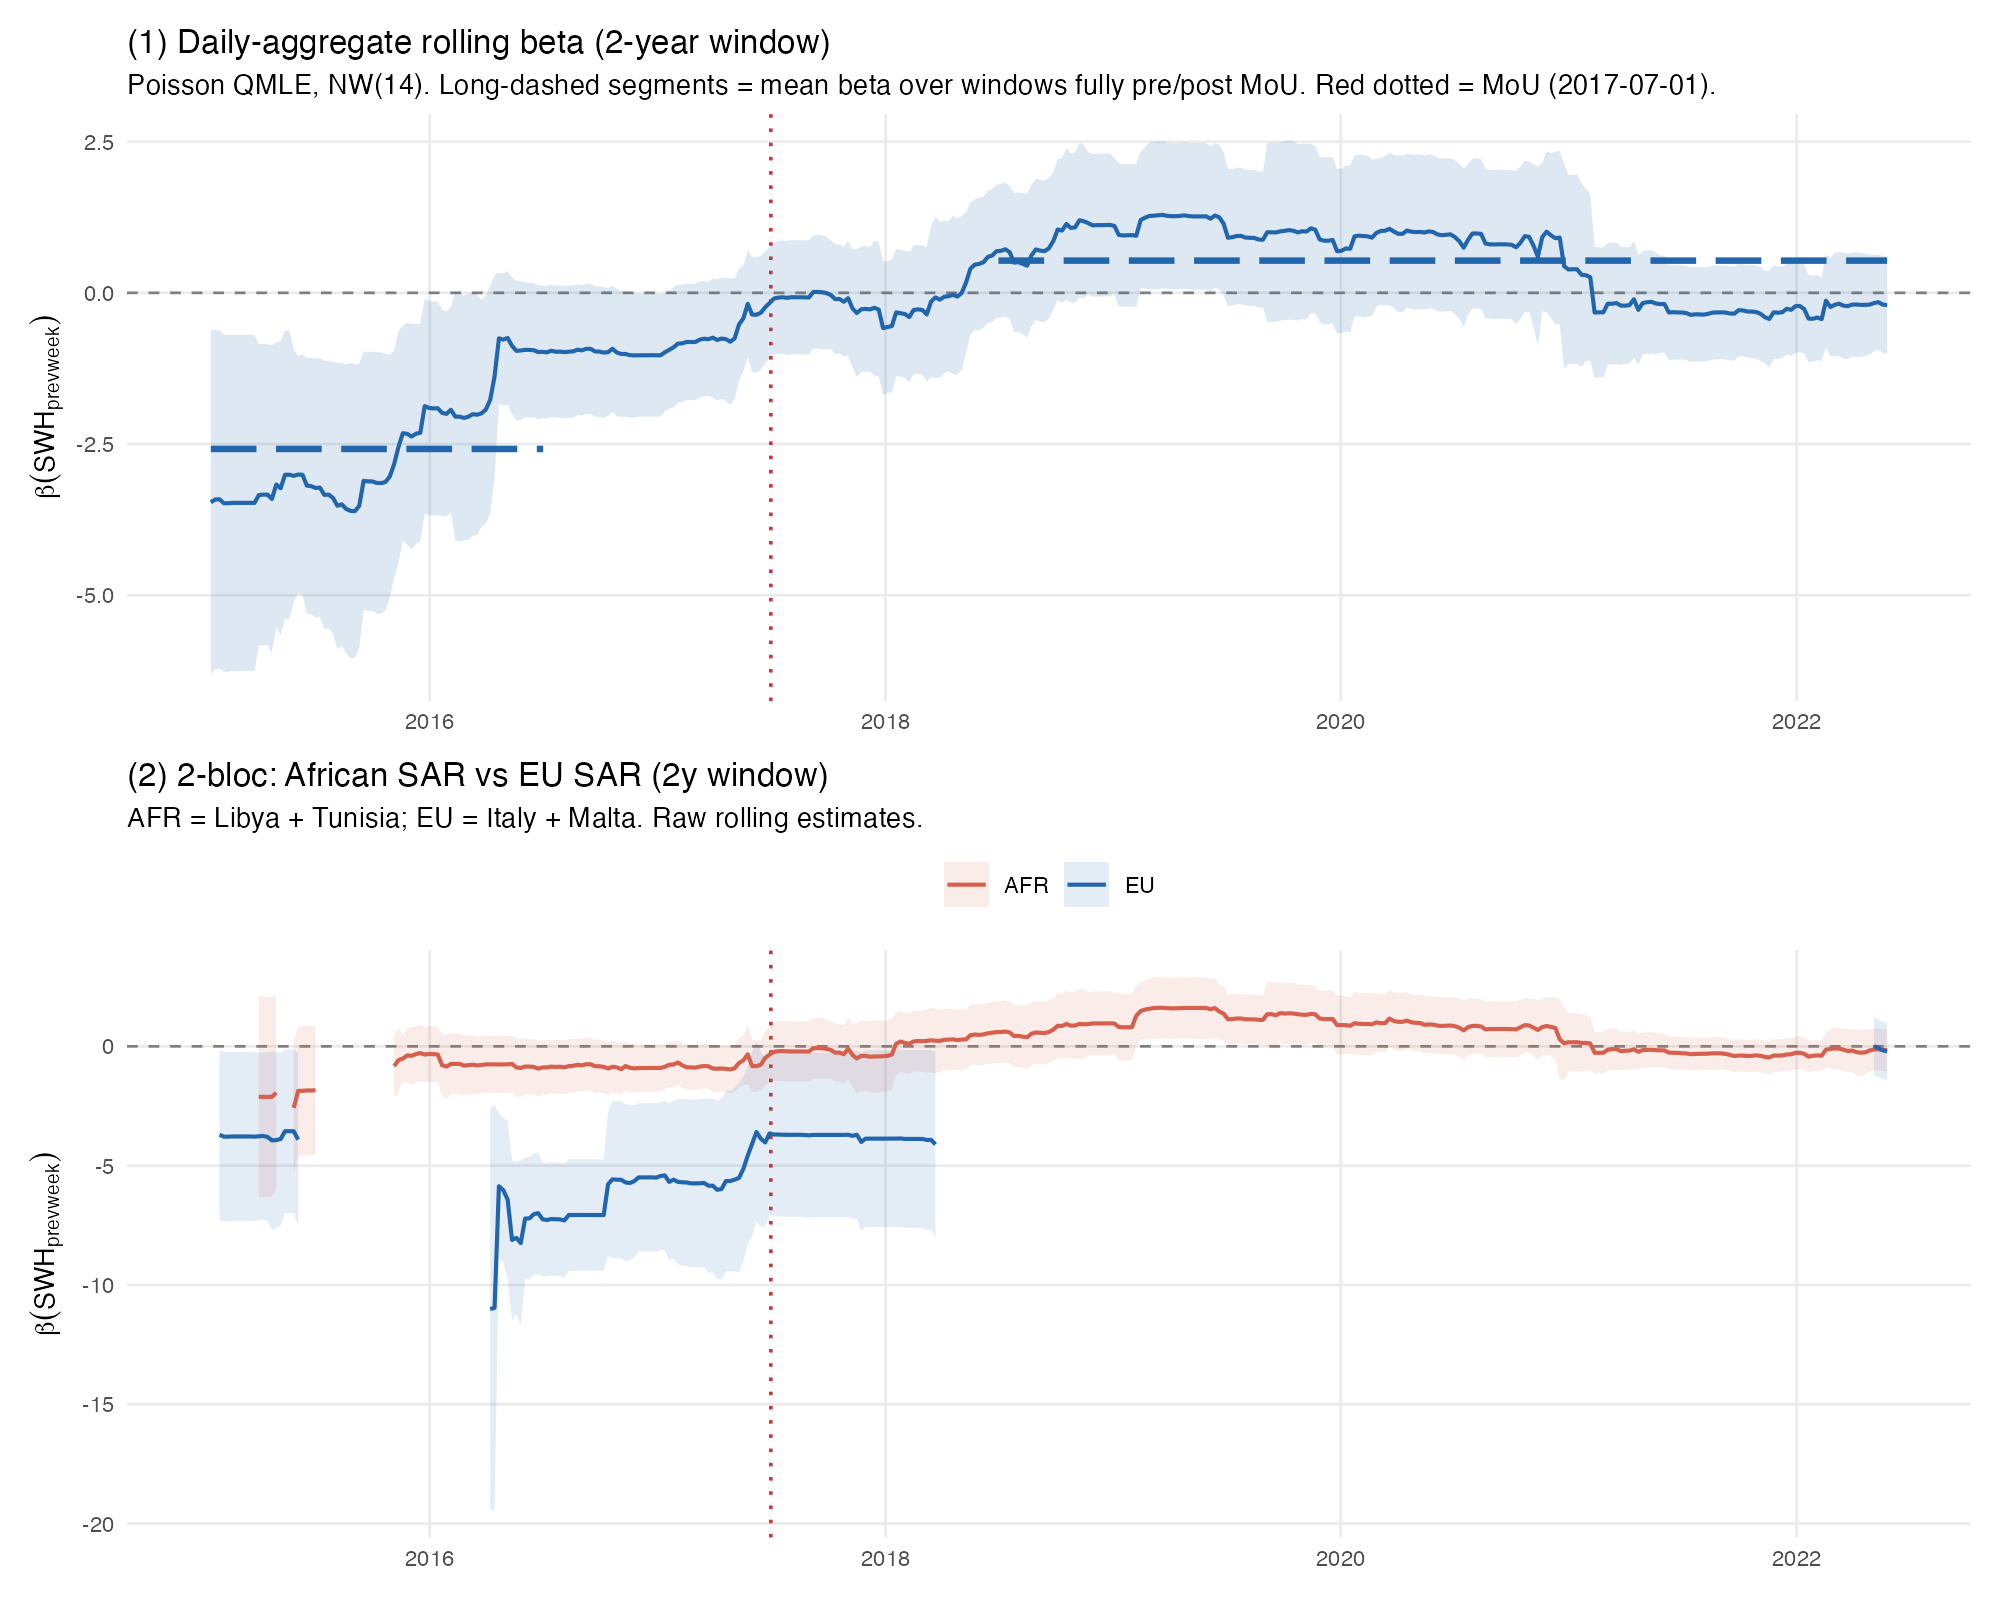
\includegraphics[width=0.95\linewidth,height=0.80\textheight,keepaspectratio]{../../output/figures/22_rolling_beta.png}
\end{center}

\footnotesize
Poisson QMLE, 730-day (2-year) window, weekly step, NW(14). The shift in
$\beta(\text{SWH})$ is \emph{smooth}, not a discrete 2017-07 break ---
consistent with gradual SAR decline rather than a MoU policy shock.
\end{frame}

% ═════════════════════════════════════════════════════════
\begin{frame}{Robustness --- Zone, FE Choice, SE Variants}

\begin{columns}[T]
\begin{column}{0.52\textwidth}
\textbf{Zone-level (AFR vs EU SAR):}
\begin{table}
\centering
\scriptsize
\begin{tabular}{lcc}
\toprule
                 & \textbf{NegBin}      & \textbf{Poisson} \\
\midrule
$\beta_3$        & $+5.02^{***}$        & $+2.96^{**}$ \\
                 & $(0.85)$             & $(0.93)$ \\
$\beta_1$        & $-4.97^{***}$        & $-2.69^{**}$ \\
\bottomrule
\end{tabular}
\end{table}
$\beta_3 > 0$ in both families; sign-flip preserved when exploiting within-day
spatial variation across SAR blocs.

\vspace{0.4em}
\textbf{FE robustness (NegBin $\beta_3$):}
\begin{itemize}
\footnotesize
  \item year $+0.72$, year+month $+0.68$ (insignificant)
  \item quarter-year $+2.01^{***}$
  \item \textbf{month-year $+2.22^{***}$ (primary)}
  \item FE matters: coarse FE leaves too little within-FE weather variation.
\end{itemize}
\end{column}
\begin{column}{0.45\textwidth}
\textbf{FE robustness:}
\begin{center}
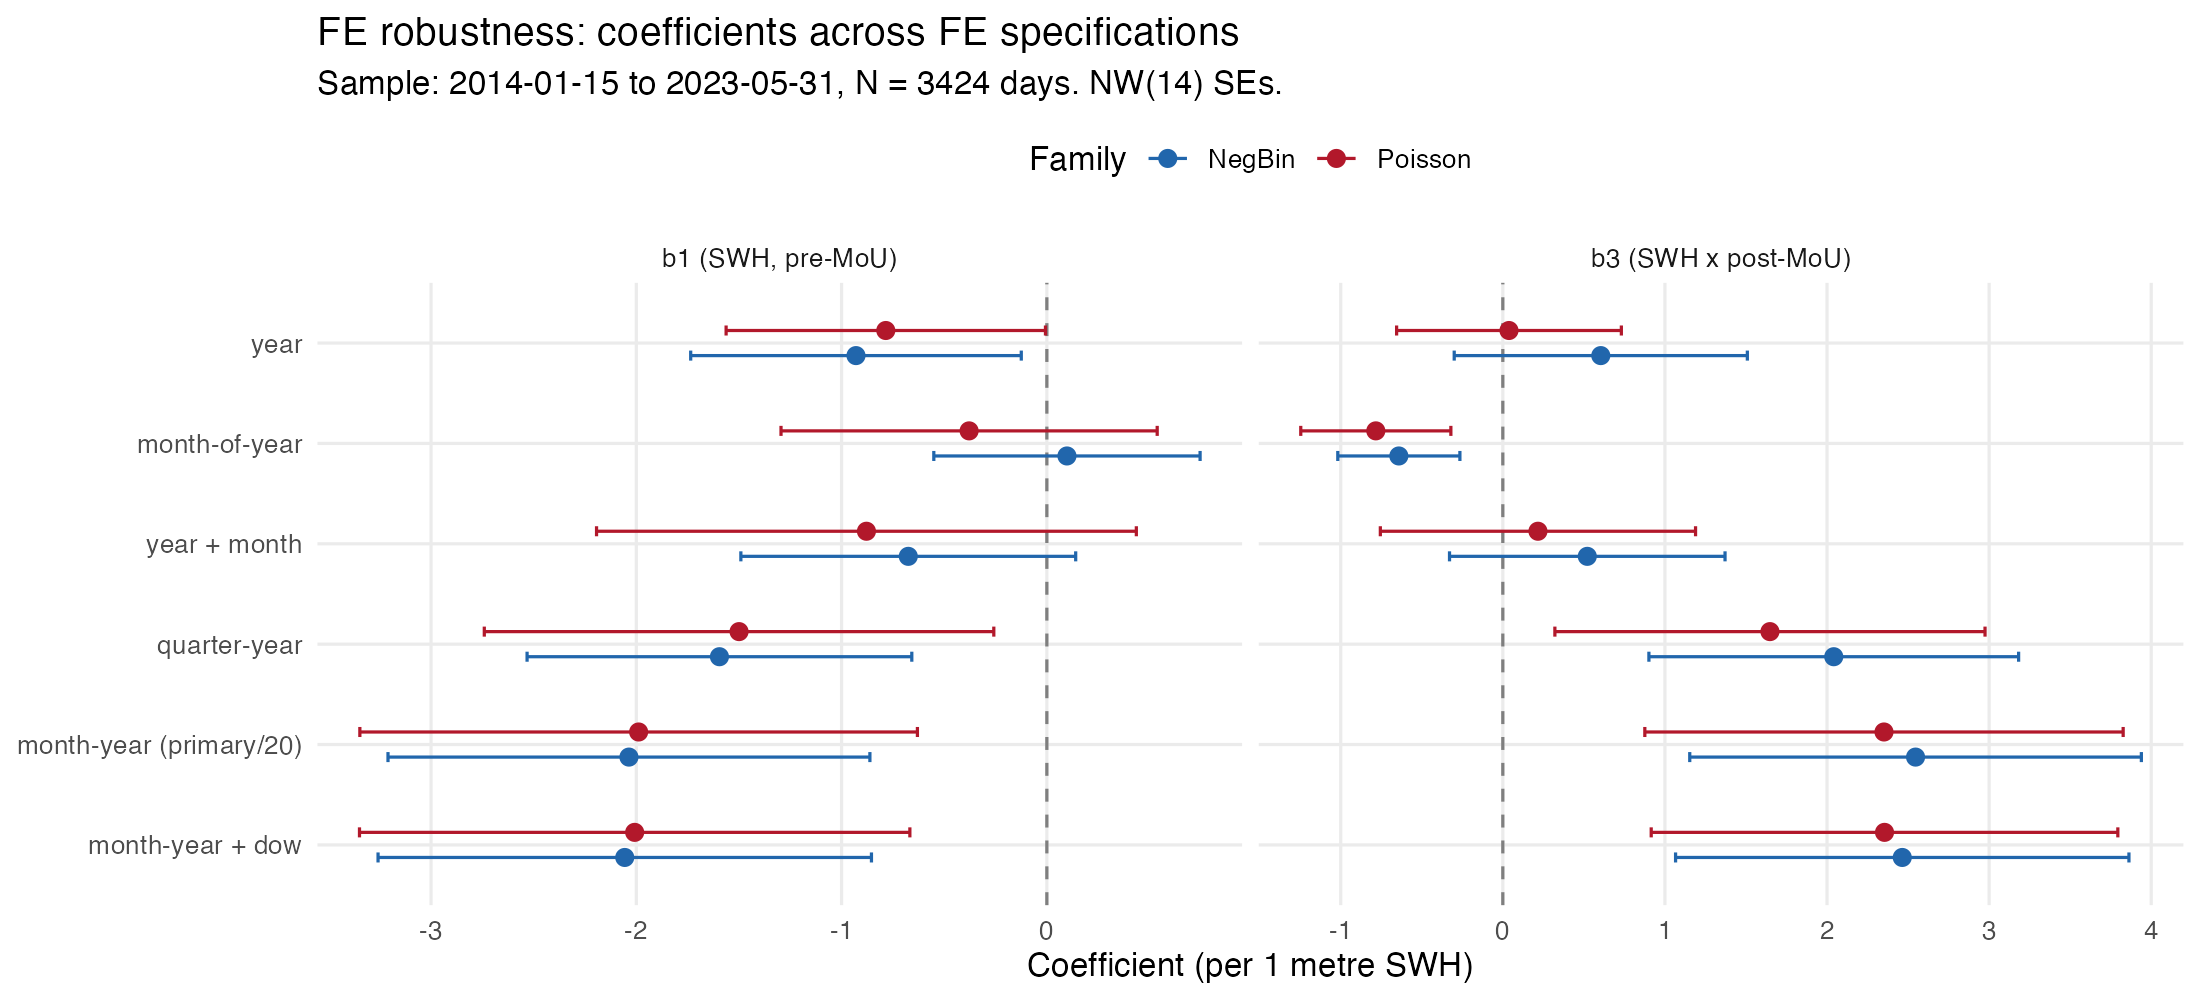
\includegraphics[width=\linewidth,height=0.72\textheight,keepaspectratio]{../../output/figures/24_fe_robustness_coefplot.png}
\end{center}
\end{column}
\end{columns}

\vspace{0.3em}
\footnotesize
Month-year FE (primary) absorb 51\% of 5-day SWH variance. Coarse FE that fail
to absorb $\text{Post}_t$ mix the interaction with a mean level shift ---
expected, noted in paper.
\end{frame}

% ═════════════════════════════════════════════════════════
\begin{frame}{Mechanism --- SAR Capacity?}

\textbf{Replace} binary $\text{Post}_t$ \textbf{with continuous moderators}
(weekly lagged averages, standardised):
\begin{itemize}
  \item SAR share $=$ Frontex SAR events / incidents
  \item Inflatable share $=$ inflatable events / incidents
  \item Persons per boat (PPB) $=$ persons / incidents
\end{itemize}

\vspace{0.3em}
\begin{table}
\centering
\small
\begin{tabular}{lccc}
\toprule
 & \textbf{SAR share} & \textbf{Inflatable share} & \textbf{PPB} \\
\midrule
Moderator main effect          & $+1.18^{***}$   & $+0.89^{**}$   & $+1.66^{***}$ \\
SWH $\times$ Moderator         & $-0.63^{**}$    & $-0.32$        & $-1.35^{***}$ \\
\bottomrule
\end{tabular}
\end{table}

\vspace{0.3em}
\footnotesize
Each column = one fit of deaths on $\text{SWH}$, a moderator $M$ (z-scored,
weekly) and their product, with month-year FE.

\emph{Main effect ($\beta_M$):} average change in deaths when $M$ is 1-SD
higher. Mostly positive --- but \textbf{confounded}: reverse causality.

\emph{Interaction ($\beta_{\text{int}}$):} change in the SWH$\to$deaths slope when
$M$ is 1-SD higher. Mechanism test --- only related to how weather translates into
deaths.

Only SAR $\times$ SWH is clearly negative ($-0.63^{**}$): 1-SD more SAR
\emph{flattens} the weather-to-deaths slope by 0.63 --- the guardrail in the
data. PPB $\times$ SWH is also negative but likely a volume-selection artefact
(rough seas deter launches, so crowded boats only appear on calmer days).
\end{frame}

% ═════════════════════════════════════════════════════════
\begin{frame}{Limitations and Takeaway}

\textbf{What the paper shows:}
\begin{enumerate}
  \item Pre-MoU: $\beta(\text{SWH}) < 0$ --- rough seas produced \emph{fewer} deaths
    (SAR coverage + voluntary departure cuts acted as a protective selection).
  \item Post-MoU: $\beta(\text{SWH})$ flips toward zero / positive.
  \item Transition is \emph{gradual} (rolling window); MoU is a marker of a
    multi-year process, not a discrete cause.
  \item SAR capacity is the mechanism most consistent with the pattern.
\end{enumerate}

\vspace{0.5em}
\textbf{Limitations:}
\begin{itemize}
  \item Panel bounded by Frontex data (2014--2023, May). Earlier years (2009--2013)
    available only via UNITED; cross-source check shows same direction.
  \item IOM deaths are under-reported (Frontex--IOM cross-check:
    $\sim\!57\%$ of on-water deaths unseen by Frontex event-level).
  \item Single corridor-wide SWH (diagnostic supports the simplification).
  \item Within-CMR identification only --- EMR/WMR control routes rejected as
    too contaminated (EU--Turkey deal, route composition).
  \item Sharp MoU date is a modelling convenience; the rolling window shows the
    true change is smooth.
\end{itemize}
\end{frame}

\end{document}
